\documentclass[xcolor=dvipsnames]{beamer}
\usetheme{Madrid}
\definecolor{VUdarkred}{rgb}{0.482, 0, 0.247}
\definecolor{VUlightgray}{rgb}{0.863, 0.863, 0.863}
\definecolor{VUdarkgray}{rgb}{0.255, 0.255, 0.255}
\definecolor{VUwhite}{rgb}{1, 1, 1}
\definecolor{VUbrightred}{rgb}{0.902, 0.255, 0.392}
%\usecolortheme[named=VU]{structure}
\setbeamercolor{palette primary}{bg=VUdarkred,fg=VUwhite}
\setbeamercolor{palette secondary}{bg=VUlightgray,fg=VUdarkgray}
\setbeamercolor{palette tertiary}{bg=VUdarkred,fg=VUwhite}
\setbeamercolor{palette quaternary}{bg=VUbrightred,fg=VUwhite}
\setbeamercolor{structure}{fg=VUbrightred} % itemize, enumerate, etc
\setbeamercolor{section in toc}{fg=VUbrightred} % TOC sections
\setbeamercolor{subsection in head/foot}{bg=VUbrightred,fg=white}

\usepackage[yyyymmdd]{datetime}
\usepackage{fontspec}
\usepackage{fontenc}
\usepackage{amssymb}
\usepackage{ulem}
\usepackage{cite}
\usepackage{multirow}
\usepackage{mathtools}
\usepackage{amsmath}
\usepackage{float}
\usepackage{graphicx}
%\usepackage{url}
\usepackage{hyperref}
\usepackage{caption}
\usepackage{appendixnumberbeamer}
%\usepackage[svgnames]{xcolor}
%\usepackage{xstring} % to define myund
\usepackage[lithuanian]{babel}
%\usepackage{lineno}
\graphicspath{ {images/} }

\renewcommand{\dateseparator}{-}
\renewcommand{\abstractname}{Santrauka}
\renewcommand{\contentsname}{Turinys}
\renewcommand{\figurename}{Pav}
\renewcommand{\refname}{Literatūra}
\renewcommand{\tablename}{Lentelė}
\renewcommand{\listfigurename}{Paveikslėlių sąrašas}
\renewcommand{\listtablename}{Lentelių sąrašas}

\DeclareCaptionLabelFormat{numfirst}{#2~#1}

\newcommand{\textblue}[1]{{\color{Blue}#1}}
\newcommand{\textred}[1]{{\color{Red}#1}}
\newcommand{\comment}[1]{\newline\textblue{#1}\newline}
\newcommand{\commentNL}[1]{\textblue{#1}\newline}
\newcommand{\commentMA}[1]{\newline\textred{#1}\newline}
\newcommand{\ttt}[1]{\texttt{#1}}
\newcommand{\pT}{\mathit{p}_{\mathrm{T}}}
\newcommand{\ET}{\mathit{E}_{\mathrm{T}}}
\newcommand{\refeqq}[1]{(\ref{#1})}
\newcommand{\Lumi}{{\cal L}_\mathrm{int}}
\newcommand{\pb}{$\mathrm{pb}$}
\newcommand{\fb}{$\mathrm{fb}$}
\newcommand{\invfb}{$\mathrm{fb}^{-1}$}
\newcommand{\invpb}{$\mathrm{pb}^{-1}$}
\newcommand{\ltq}[1]{{\quotedblbase{}#1\textquotedblleft{}}}
\newcommand{\WJets}{\mathit{W}+\mathrm{Jets}}
\newcommand{\emu}{\mathit{e}\mu}
\newcommand{\ee}{\mathit{ee}}
\newcommand{\mumu}{\mu\mu}
\newcommand{\WW}{\mathit{WW}}
\newcommand{\WWpm}{\mathit{W^{\,+}\!W^{\,-}}}
\newcommand{\ZZ}{\mathit{ZZ}}
\newcommand{\WZ}{\mathit{WZ}}
\newcommand{\gJets}{\gamma\! +\!\mathrm{Jets}}
\newcommand{\DYee}{\mathrm{DY} \! \rightarrow \! \mathit{ee}}
\newcommand{\DYtau}{\mathrm{DY} \! \rightarrow \! \tau\tau}
\newcommand{\dtW}{\mathit{tW}\! + \! \overline{\mathit{t}}\mathit{W}}
\newcommand{\QCD}{\mathit{QCD}}
\newcommand{\ttbar}{\mathit{t}\overline{\mathit{t}}}
\newcommand{\tbarW}{\overline{\mathit{t}}\mathit{W}}
\newcommand{\tW}{\mathit{tW}}
\newcommand{\MC}{\mathrm{MC}}
\newcommand{\Data}{\mathrm{Data}}



\title[Drell-Yan analizė]{Drell-Yan proceso tyrimas analizuojant CERN CMS eksperimento 2016 metų protonų susidūrimų duomenis}
\subtitle{Magistrantūros studijų mokslo tiriamosios praktikos darbas}
\author[M.\ Ambrozas]
{Darbą atliko Marijus Ambrozas\\ Vadovas dr.\ Andrius Juodagalvis}
\institute[VU FF]
{
  Vilniaus universitetas, Fizikos fakultetas
}
\date[2019-01-25]{2019 m.\ sausio 25 d.}
%\titlegraphic{
\includegraphics[width=1.75cm]{VU_Logo_bordo.png}\hspace*{0.1cm}
%			  
\includegraphics[width=1.75cm]{VUFF-logo1.jpg}\hspace*{0.1cm}\includegraphics[width=1.75cm]{VUTFAI-logo.pdf}}
\titlegraphic{
\includegraphics[width=4cm]{logo_lt.png}\hspace*{0.1cm}
			  \includegraphics[width=2cm]{VUTFAI-logo.pdf}}

\begin{document}
\frame{\titlepage}


\section{Įvadas}

\begin{frame}
	\subsection{Drell-Yan procesas}
	\frametitle{Drell-Yan procesas}
	\begin{itemize}
		\item Drell-Yan procesas -- kvarko ir antikvarko anihiliacija, kurios rezultatas -- leptono ir antileptono pora:
		$\mathit{q}\bar{\mathit{q}}\rightarrow \gamma^{*}/\mathit{Z}\rightarrow \mathit{l^{\, +}\! l^{\, -}}$
		($\mathrm{DY}\!\rightarrow\!\mathit{l^{\, +}\! l^{\, -}}$);
		\item Šiame darba nagrinėtos galutinės būsenos -- elektronų bei miuonų poros;
	\end{itemize}
	\begin{minipage}{0.45\textwidth}
		\begin{figure}[H]
			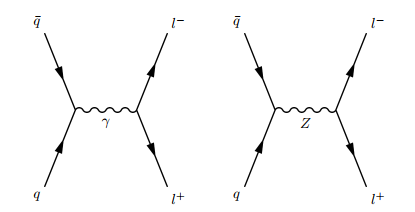
\includegraphics[width=\textwidth]{DYprocess.PNG}
		\end{figure}
		\begin{itemize}
			\item \small Vienas iš matuojamų pasiskirstymų -- diferencialinis sklaidos skerspjūvis
			$\mathrm{d}\sigma/\mathrm{d}\mathit{m}_{\mathit{ll}}$.;
		\end{itemize}
	\end{minipage}
	\hfill
	\begin{minipage}{0.54\textwidth}
		\vspace{-0.2cm}
		\begin{figure}[H]
			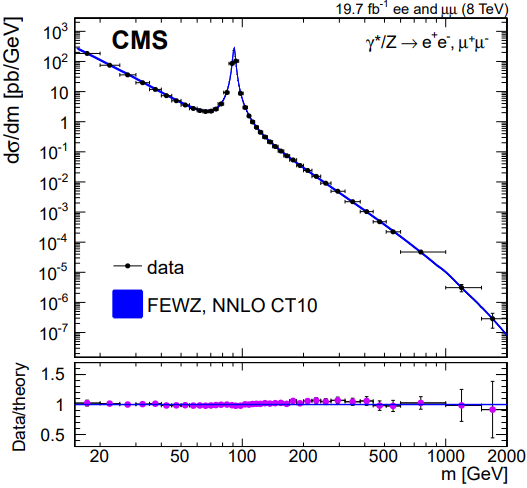
\includegraphics[width=0.8\textwidth]{DYeeCS.PNG}
		\end{figure}
		\vspace{-0.4cm}
		\tiny\centering(CMS Collaboration. CMS-PAS-SMP-14-003, 2014.)
	\end{minipage}
\end{frame}


\begin{frame}
	\subsection{Drell-Yan proceso triukšmo įvykiai}
	\frametitle{Drell-Yan proceso triukšmo įvykiai}
	% Šviesos greičiu lekiančių dalelių gyvavimo trukmė laboratorinėje sistemoje pailgėja.
	%Pvz., miuonai nėra stabilūs. Taip pat hadronai.
	%Standartinis ECAL triukšmas - neutralūs pionai, skylantys į du fotonus.
	Dalelių detektoriai registruoja ilgai gyvuojančias po protonų susidūrimo susidariusias daleles.

	\medskip

	\begin{itemize}
		% Signalas - mus dominantis procesas
		\item \textbf{Signalas} - mus dominančio proceso galutinė būsena ($\mathrm{DY}\!\rightarrow\!\mathit{e^{+}\! e^{-}}$ arba
		$\mathrm{DY}\!\rightarrow\!\mathit{\mu^{+}\! \mu^{-}}$);
		\item \textbf{Triukšmas} - bet kuris kitas procesas, galintis turėti tokią pačią galutinę būseną, kaip ir signalas;\\[5mm]
		% Būtų gerai triukšmus išdėlioti pagal dažnumą (didėjančia arba mažėjančia tvarka)
		\item Pagrindiniai triukšmai:\\
		$\mathit{ZZ}$, $\mathit{tW}$, $\bar{\mathit{t}}\mathit{W}$, $\mathit{WZ}$, $\mathit{WW}$, $\mathit{t}\bar{\mathit{t}}$,
		$\mathrm{DY}\!\rightarrow\!\mathit{\tau^{+\,}\!\tau^{-}}$, $\WJets$, $\mathit{QCD}$;
		\item Triukšmo įvykių skaičiaus įvertinimo būdai:
		\begin{enumerate}
			\item Monte Carlo (MC) modeliavimas;
			\item Matavimu grįsti metodai ($\emu$ metodas);
		\end{enumerate}
	\end{itemize}

	\medskip

	Siekiant išvengti su matavimu tiesiogiai nesusijusių neapibrėžtumų yra naudojami matavimu grįsti metodai.
	% Pvz., dėl prastai sumodeliuoto detektoriaus atsako
\end{frame}


\begin{frame}
	\section{Darbo tikslas}
	\frametitle{Darbo tikslas}
	Šio darbo tikslas:
	\begin{itemize}
		\item Iš didelio duomenų rinkinio išrinkti su Drell-Yan procesu siejamus įvykius;
		\item Palyginti, kaip gerai modeliuotas leptonų poros invariantinės masės pasiskirstymas atitinka išmatuotąjį;
		\item $\emu$ metodu įvertinti Drell-Yan proceso triukšmo įvykių skaičių;
	\end{itemize}
	\vspace{0.5cm}
	\small Darbe buvo naudojami $2016$ metais CERN CMS detektoriaus užregistruoti $13 \; \mathrm{TeV}$ energijos
	protonų susidūrimų duomenys, atitinkantys $35.9 \; \mathrm{fb}^{-1}$ integruotąjį šviesį.
\end{frame}


\begin{frame}
	\frametitle{Darbo schema}
	\begin{enumerate}
		\item Įvykių atranka;
		\item Modeliuotų įvykių normavimas ir pataisų pritaikymas;
%		\begin{itemize}
%        	\item Normavimas pagal integruotą šviesį;
%			\item Normavimas pagal protonų susidūrimų tankį;
%			\item Matavimo skalės bei efektyvumų pataisų taikymas;
%		\end{itemize}
		\item matavimo ir modeliavimo palyginimas;
		\item $\emu$ metodo taikymas:
%		\begin{itemize}
%        	\item Pradinė atranka;
%			\item Netikrų $\emu$ įvykių (\ltq{$\emu$ triukšmų}) įskaitymas;
%		\end{itemize}
	\end{enumerate}
\end{frame}

\begin{frame}
	\section{Įvykių atranka}
	\frametitle{Įvykių atranka}
	\begin{enumerate}
		\item Pradiniai eksperimentinių ir modeliuotų duomenų rinkiniai užima $14\; \mathrm{TB}$ ir yra saugomi
		Pietų korėjos \textit{Tier3} duomenų centre;
		\item Protonų susidūrimo įvykiai buvo atrenkami vadovaujantis tokiais kriterijais:
	\end{enumerate}
	\vspace{-0.2cm}
	\begin{center}
		\footnotesize
		\begin{tabular}{|c|c|}
			\hline
			$\ee$ įvykiai & $\mumu$ įvykiai \\
			\hline\hline
			\multirow{4}{6em}{\centering\textbf{Trigeris:} \ttt{Ele23\_Ele12}} & \textbf{Trigeris:} \\
			& \ttt{HLT\_IsoMu24} arba \ttt{HLT\_TkMu24} \\
			& (bent vienas miuonas turi būti \\
			& tas, kuris aktyvavo trigerį) \\
			\hline
			
			$\mathit{p}_{\mathrm{T}}^{\mathrm{Lead}} > 28 \; \mathrm{GeV}$, &
				\multirow{4}{10em}{\centering$\mathit{p}_{\mathrm{T}}^{\mathrm{Lead}} > 28 \; \mathrm{GeV}$,
				$\mathit{p}_{\mathrm{T}}^{\mathrm{Sublead}} > 17 \; \mathrm{GeV}$,
				$|\eta| < 2.4$} \\
			$\mathit{p}_{\mathrm{T}}^{\mathrm{Sublead}} > 17 \; \mathrm{GeV}$, & \\
			$|\eta_{\mathrm{SC}}| < 2.4$, & \\
			\textbf{išskyrus} $1.4442 < |\eta_{\mathrm{SC}}| < 1.566$ & \\
			\hline
			\textit{Electron MediumID} & \textit{Muon TightID}, $\mathit{I}_{\mathrm{PF}}^{\mathrm{Rel.}} < 0.15$  \\
			\hline
			\multirow{4}{13em}{\centering Visus išvardintus kriterijus turi atitikti lygiai du elektronai} & Du miuonai su mažiausiu bendros \\
			& viršūnės aproksimacijos $\chi^2 < 20$. \\
			& Kampas tarp miuonų trajektorijų \\
			& $\alpha < \pi - 0.005 \; \mathrm{rad}$ \\
			\hline
		\end{tabular}
	\end{center}
\end{frame}

\begin{frame}
	\frametitle{Modeliuotų įvykių normavimas, pataisos}		
	Su atrinktais modeliuotais duomenimis buvo atliekamos šios operacijos:
	\begin{enumerate}
		\item Normavimas pagal išmatuotą integruotą šviesį;
		\item Normavimas pagal protonų susidūrimų tankį;
		\item Trigerių suveikimo, leptonų atpažinimo, atkūrimo, bei miuonų atskirumo įvertinimo pataisos.
	\end{enumerate}
	Su eksperimentiniais ir modeliuotais įvykiais buvo atliekamos elektronų energijos matavimo skalės bei miuonų skersinio
	impulso skalės pataisos.
\end{frame}

\begin{frame}
	\section{emu metodo veikimo principas}
	\frametitle{$\emu$ metodo veikimo principas}
	\large $\emu$ metodas leidžia įvertinti indėlį tokių triukšmų, kurių galutinė būsena gali susidėti iš tiek tos pačios,
	tiek skirtingų rūšių leptonų.
	\medskip
	\normalsize
	\begin{itemize}
		\item Pagrindiniai yra šie triukšmai: $\ZZ$, $\tW$, $\tbarW$, $WZ$, $\WW$, $\ttbar$, $\DYtau$.
		\bigskip
		\item Pvz., mus dominančios $\WW$ būsenos (be skilimo į $\tau$ leptoną):\\[3mm]
		$\WWpm\!\!\rightarrow\!\mathit{e^{+}\!e^{-}}$, $\WWpm\!\!\rightarrow\!\mathit{e^{+}\!\mu^{-}}$,
		$\WWpm\!\!\rightarrow\!\mathit{\mu^{+}\!e^{-}}$, $\WWpm\!\!\rightarrow\!\mu^{+}\!\mu^{-}$;
		\vspace{0.3cm}
		\item Iš modeliavimo galima apskaičiuoti $\ee$ ir $\emu$ įvykių santykį $\mathit{N}_{\ee}^{\MC}/\mathit{N}_{\emu}^{\MC}$;
		\item Tikėdamiesi, kad $\mathit{N}_{\ee}^{\MC}/\mathit{N}_{\emu}^{\MC}=\mathit{N}_{\ee}^{\Data}/\mathit{N}_{\emu}^{\Data}$,
		galime įvertinti $\mathit{N}_{\ee}^{\Data}$:
		\begin{equation*}
			\mathit{N_{ee}^{\mathrm{Įvert.}}} = \frac{\mathit{N_{ee}^{\mathrm{MC}}}}{\mathit{N_{e\mu}^{\mathrm{MC}}}}
												\mathit{N_{e\mu}^{\mathrm{Data}}} \; .
		\end{equation*}
		Tas pats galioja ir $\mumu$ įvykiams.
	\end{itemize}
\end{frame}

\begin{frame}
	\section{Įvykių atrankos rezultatai}
	\frametitle{Įvykių atrankos rezultatai}
	\begin{itemize}
		\item Atranką praėję įvykiai buvo įrašyti į naujus duomenų failus;
		\item Atrankos procesas trunka apie $5$ valandas;
		\item Atrinkti duomenų failai bendrai užima apie $14 \; \mathrm{GB}$;
		\item Tolimesni skaičiavimai ir grafikų gavimas iš atrinktų duomenų failų užtrunka $2-3$ minutes.
	\end{itemize}
\end{frame}

\begin{frame}
	\section{ee matavimo ir modeliavimo palyginimas}
	\frametitle{Matavimo ir modeliavimo palyginimas}
	CMS detektoriaus užregistruotas ir modeliuotas $\ee$ invariantinės masės pasiskirstymai prieš ir po pataisų pritaikymo:
	\begin{minipage}{0.49\textwidth}
		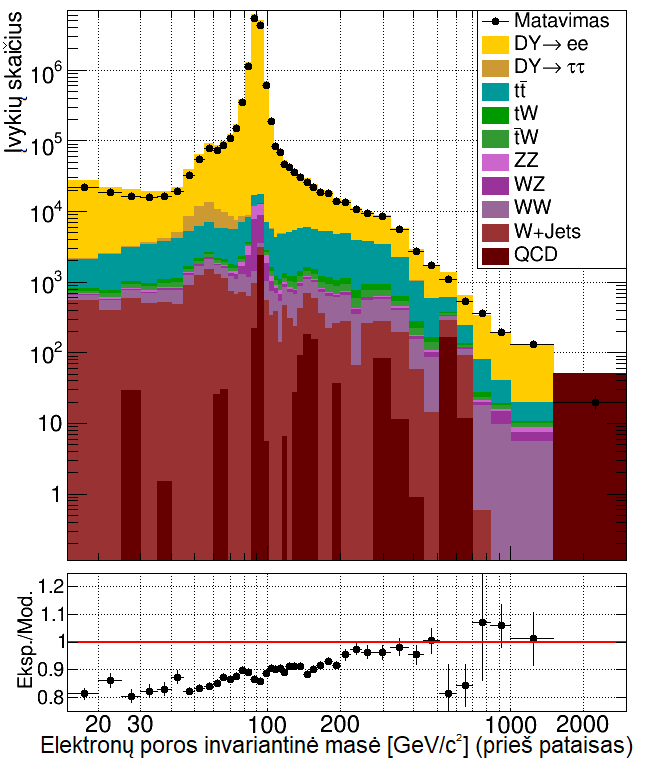
\includegraphics[width=\linewidth]{eeMassBefore_SMALL.png}
	\end{minipage}
	\hfill
	\begin{minipage}{0.49\textwidth}
		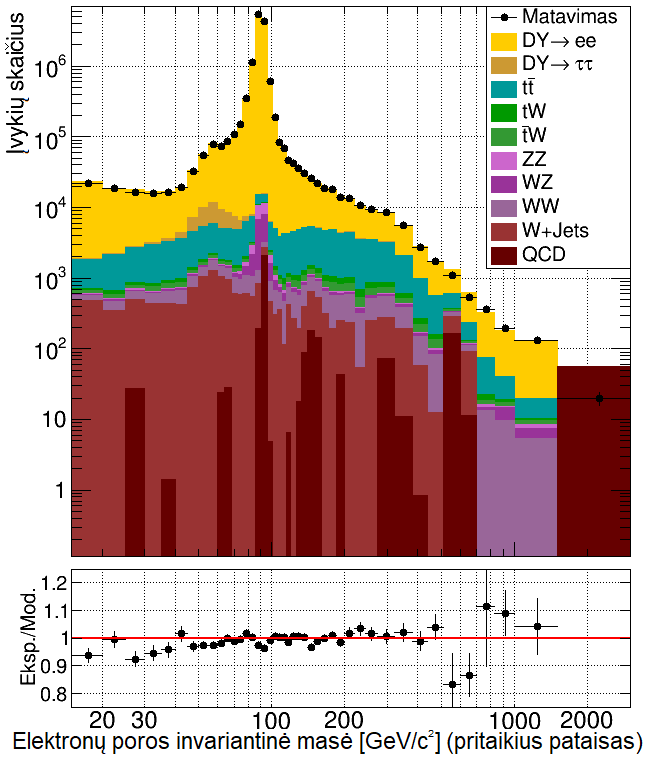
\includegraphics[width=\linewidth]{eeMassAfter_SMALL.png}
	\end{minipage}
\end{frame}

\begin{frame}
	\section{mumu matavimo ir modeliavimo palyginimas}
	\frametitle{Matavimo ir modeliavimo palyginimas}
	CMS detektoriaus užregistruotas ir modeliuotas $\mumu$ invariantinės masės pasiskirstymai prieš ir po pataisų pritaikymo:
	\begin{minipage}{0.49\textwidth}
		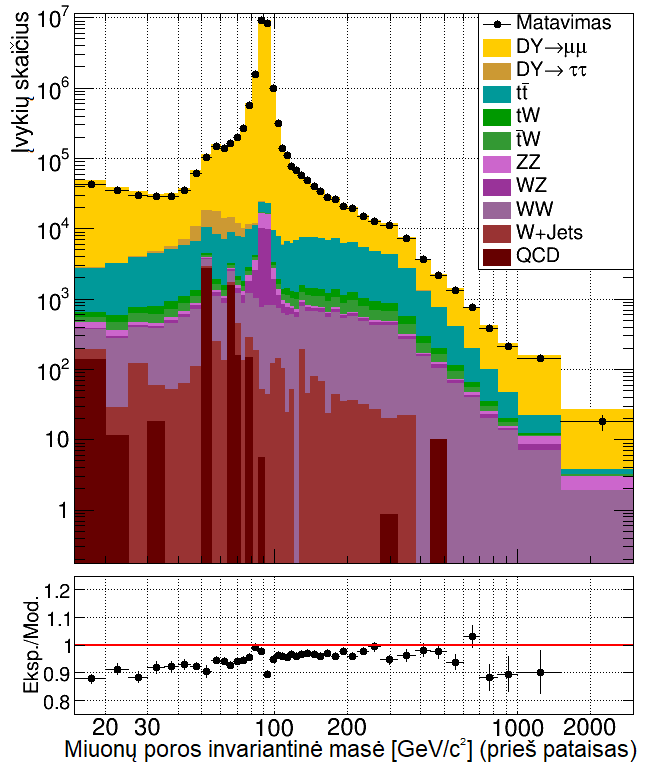
\includegraphics[width=\linewidth]{mumuMassBefore_SMALL.png}
	\end{minipage}
	\hfill
	\begin{minipage}{0.49\textwidth}
		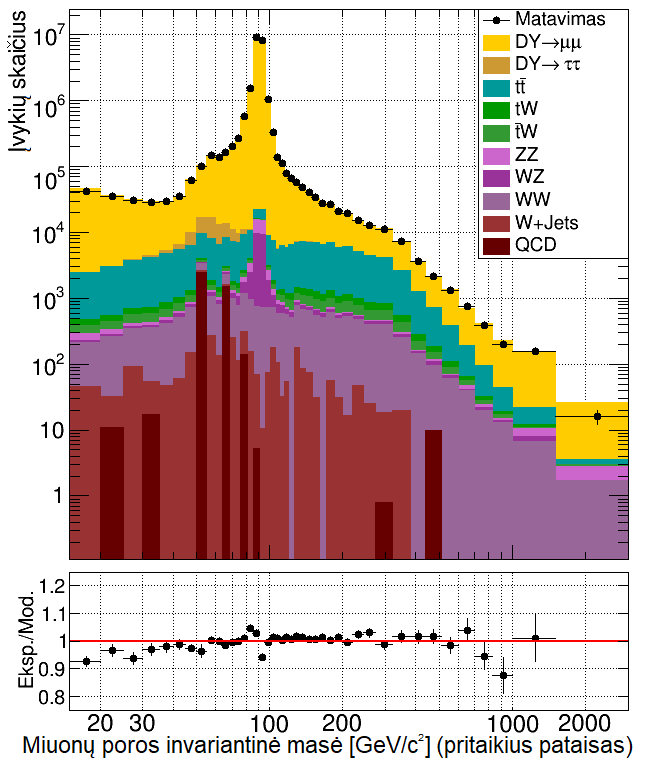
\includegraphics[width=\linewidth]{mumuMassAfter_SMALL.png}
	\end{minipage}
\end{frame}

\begin{frame}
	\section{Triukšmų įskaitymas}
	\frametitle{$\emu$ metodo taikymas\\ \normalsize Panašių į $\emu$ įvykių (\ltq{$\emu$ triukšmų}) įskaitymas}
	Netikrų $\emu$ įvykių skaičius buvo įvertinamas pasinaudojant įvykiais, kuriuose elektronas ir miuonas buvo vienodo krūvio:
	\begin{minipage}{0.44\textwidth}
		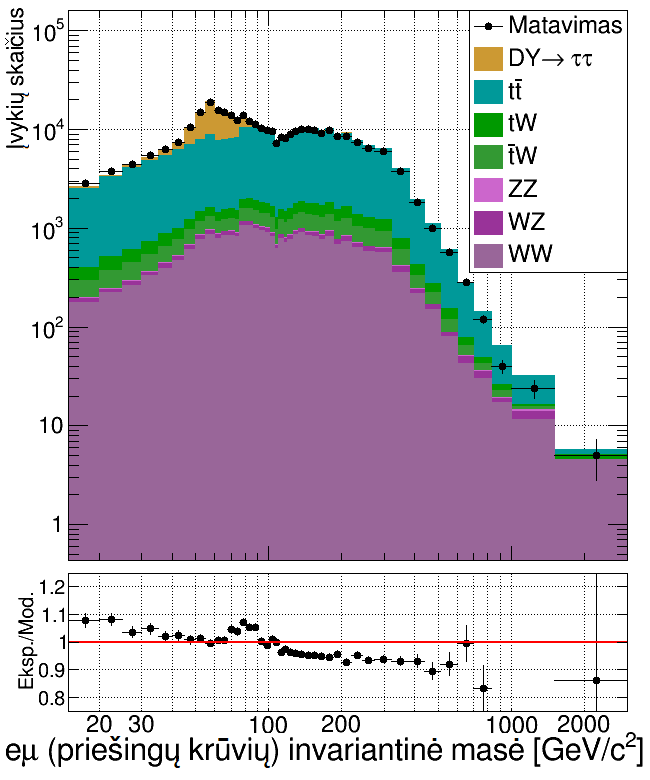
\includegraphics[width=\linewidth]{emuMassOS_SMALL.png}
	\end{minipage}
	\hfill
	\begin{minipage}{0.44\textwidth}
		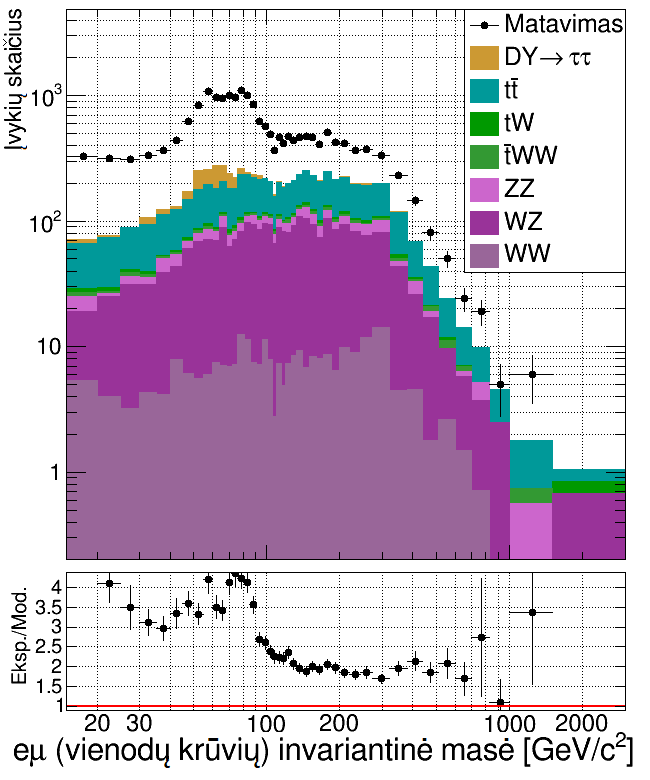
\includegraphics[width=\linewidth]{emuMassSS_SMALL.png}
	\end{minipage}
\end{frame}

\begin{frame}
	\frametitle{$\emu$ metodo taikymas\\ \normalsize Panašių į $\emu$ įvykių (\ltq{$\emu$ triukšmų}) įskaitymas}
	\begin{minipage}{0.46\textwidth}
		Prieš netikrų $\emu$ įvykių įvertinimą:
		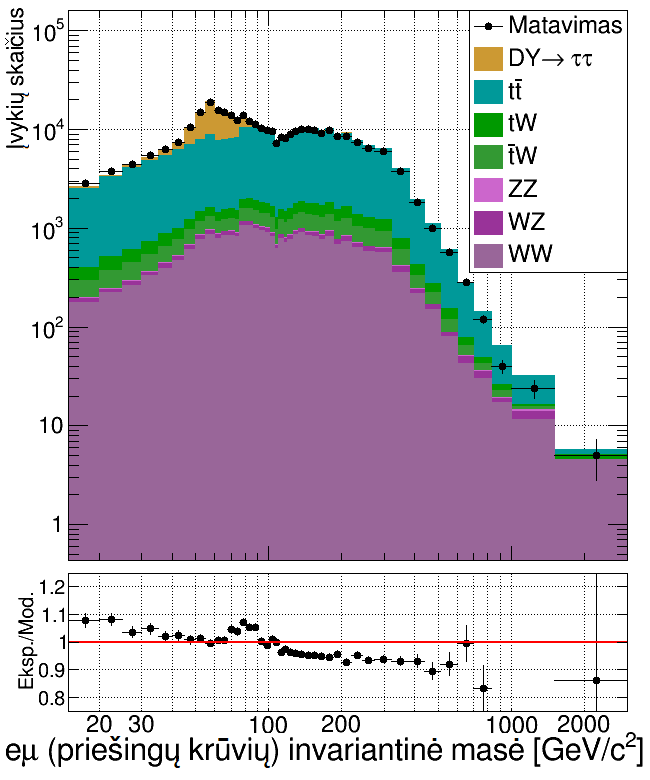
\includegraphics[width=\linewidth]{emuMassOS_SMALL.png}
	\end{minipage}
	\hfill
	\begin{minipage}{0.46\textwidth}
		Po netikrų $\emu$ įvykių įvertinimo:
		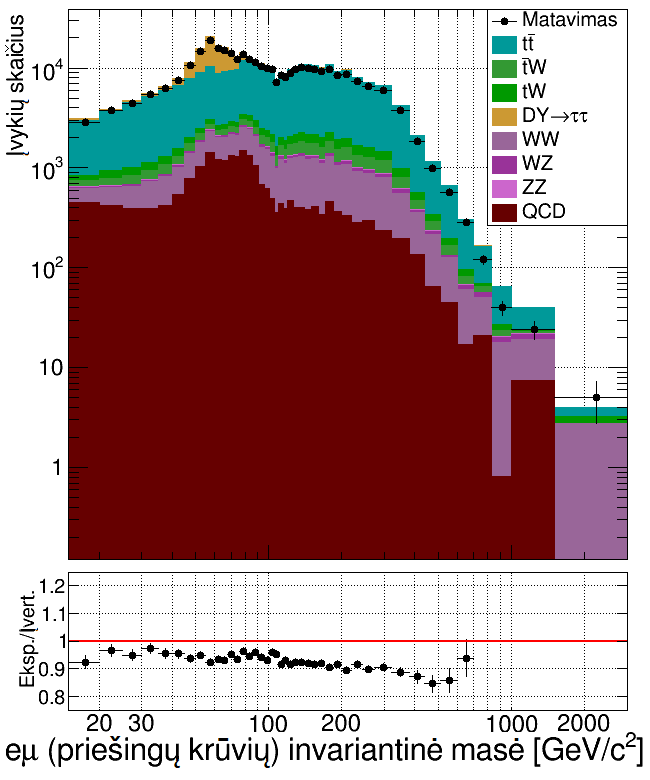
\includegraphics[width=\linewidth]{emuWQCD_SMALL.png}
	\end{minipage}
\end{frame}


\begin{frame}
	\section{Triukšmų įskaitymas}
	\frametitle{$\emu$ metodo taikymas\\ \normalsize Panašių į $\emu$ įvykių (\ltq{$\emu$ triukšmų}) įskaitymas}
	\begin{minipage}{0.44\textwidth}
		Prieš netikrų $\emu$ įvykių įvertinimą:
		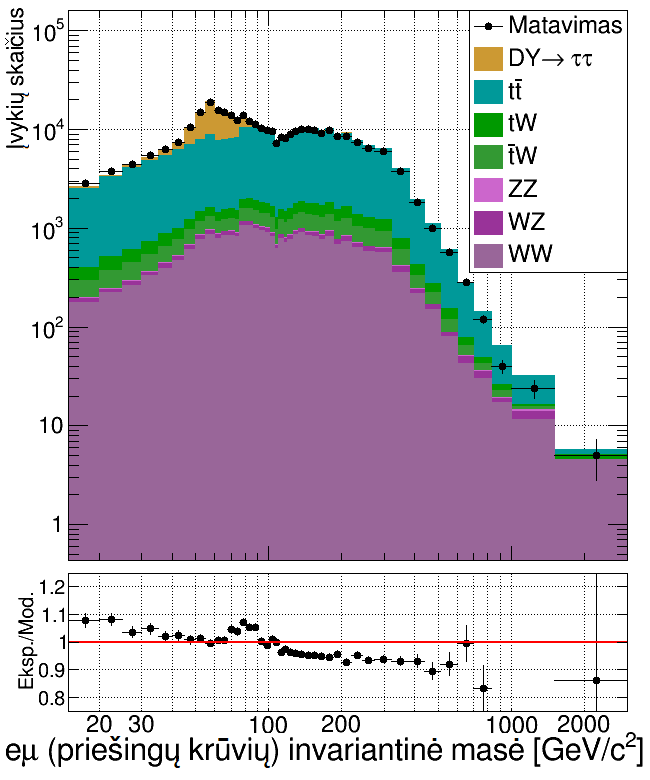
\includegraphics[width=\linewidth]{emuMassOS_SMALL.png}
	\end{minipage}
	\hfill
	\begin{minipage}{0.44\textwidth}
		Po netikrų $\emu$ įvykių įvertinimo:
		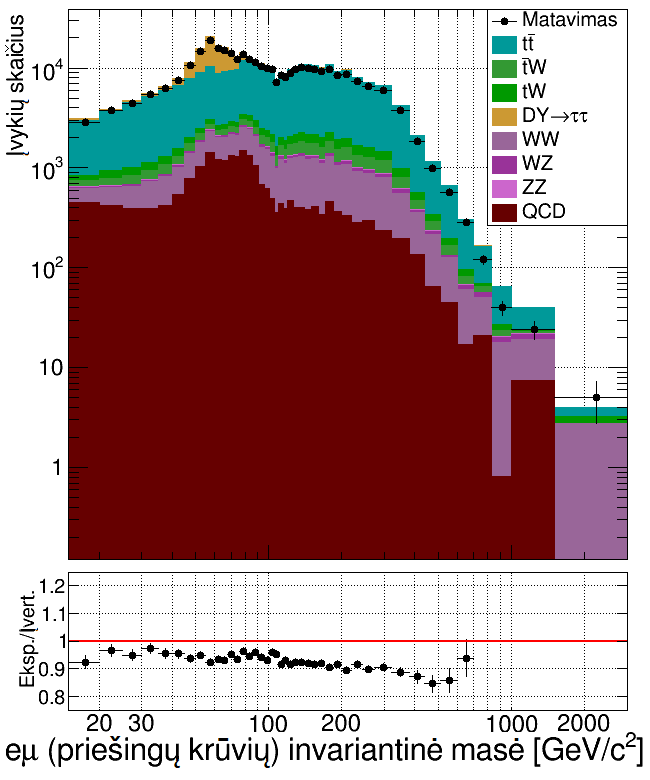
\includegraphics[width=\linewidth]{emuWQCD_SMALL.png}
	\end{minipage}
\end{frame}


\begin{frame}
	\section{emu metodo rezultatai}
	\frametitle{$\emu$ metodo rezultatai}
	$\emu$ metodu įvertinti Drell-Yan triukšmo procesų $\ee$ ir $\mumu$ galutinių būsenų invariantinių masių pasiskirstymai.
	
	\begin{minipage}{0.46\textwidth}
		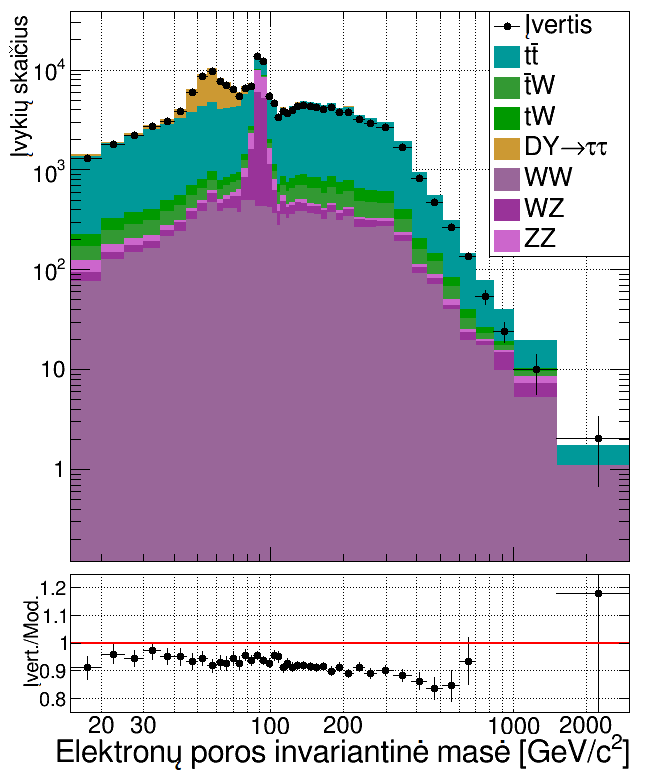
\includegraphics[width=\linewidth]{eeMassEst_SMALL.png}
	\end{minipage}
	\hfill
	\begin{minipage}{0.46\textwidth}
		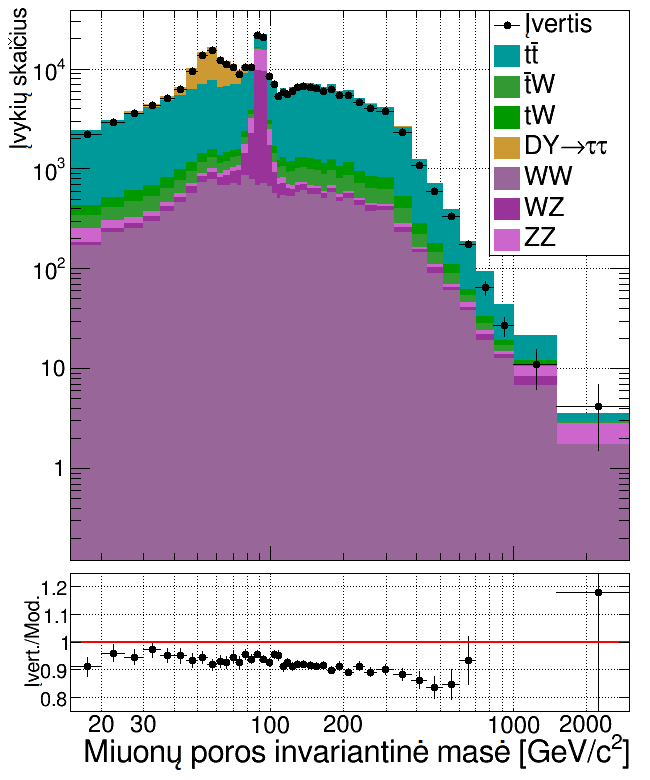
\includegraphics[width=\linewidth]{mumuMassEst_SMALL.png}
	\end{minipage}
\end{frame}


\begin{frame}
	\section{ee galutinis rezultatas}
	\frametitle{Galutinis rezultatas: $\ee$}
	Galutinis rezultatas: CMS detektoriaus užregistruotų, modeliuotų, bei $\emu$ metodu įvertintų $\ee$ įvykių invariantinės
	masės pasiskirstymas:
	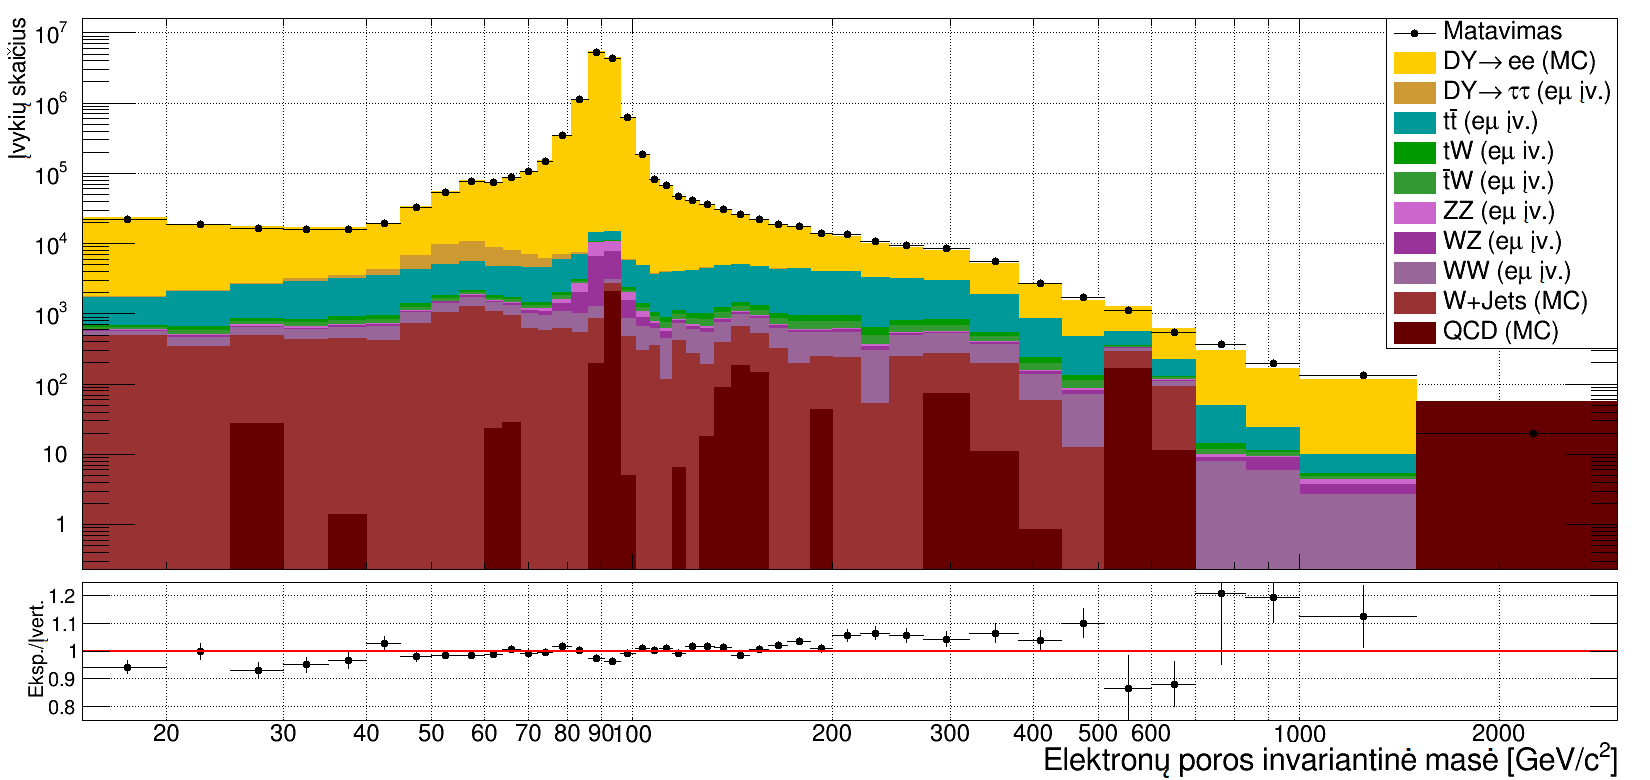
\includegraphics[width=\textwidth]{eeMassFinal_BIG.png}
\end{frame}

\begin{frame}
	\section{mumu galutinis rezultatas}
	\frametitle{Galutinis rezultatas: $\mumu$}
	Galutinis rezultatas: CMS detektoriaus užregistruotų, modeliuotų, bei $\emu$ metodu įvertintų $\mumu$ įvykių invariantinės
	masės pasiskirstymas:
	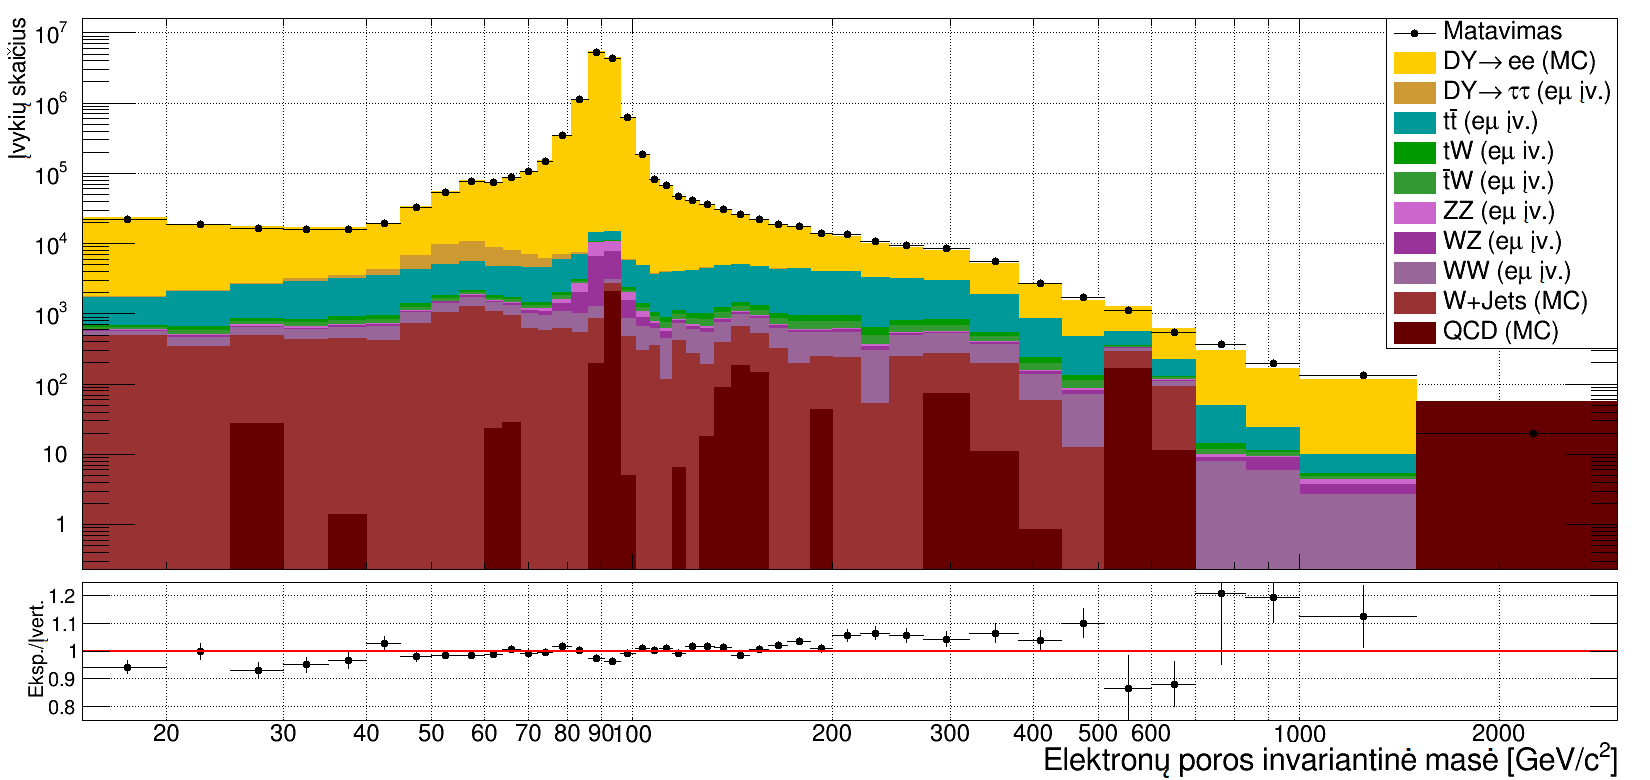
\includegraphics[width=\textwidth]{eeMassFinal_BIG.png}
\end{frame}


\begin{frame}
\section{Išvados}
\frametitle{Išvados}
\begin{itemize}
\item Įvertinus Drell-Yan proceso triukšmo įvykių skaičių $\emu$ metodu, gautas pilnutinis įvykių skaičius buvo artimesnis užregistruotajam CMS detektoriumi, nei naudojant vien tik modeliavimo įvertį, tad $\emu$ metodo naudojimas yra naudingas.
\item $\emu$ metodo skaičiavimuose atsižvelgus į panašių į $\emu$ procesų egzistavimą galima pagerinti įvertį.
\item $\emu$ metodo tikslumas, lyginant su modeliuotu įverčiu, yra žemesnis, tačiau gautas įvykių skaičius yra patikimesnis, nes modeliavime yra nežinomų neapibrėžtumų.
\end{itemize}
\end{frame}

\begin{frame}
\begin{center}
\huge Ačiū už dėmesį
\end{center}
\end{frame}

\appendix

\section{Papildoma informacija}

\begin{frame}
\subsection{CMS detektorius}
\frametitle{Papildoma informacija\\ \small CMS detektorius}
CMS -- kompaktiškasis miuonų solenoidas. Tai plačios paskirties dalelių detektorius, registruojantis LHC vykstančius protonų susidūrimus. Detektorius yra cilindro formos ir yra sudarytas iš sluoksniais išdėliotų subdetektorių, skirtų registruoti skirtingas daleles.
\begin{figure}[H]
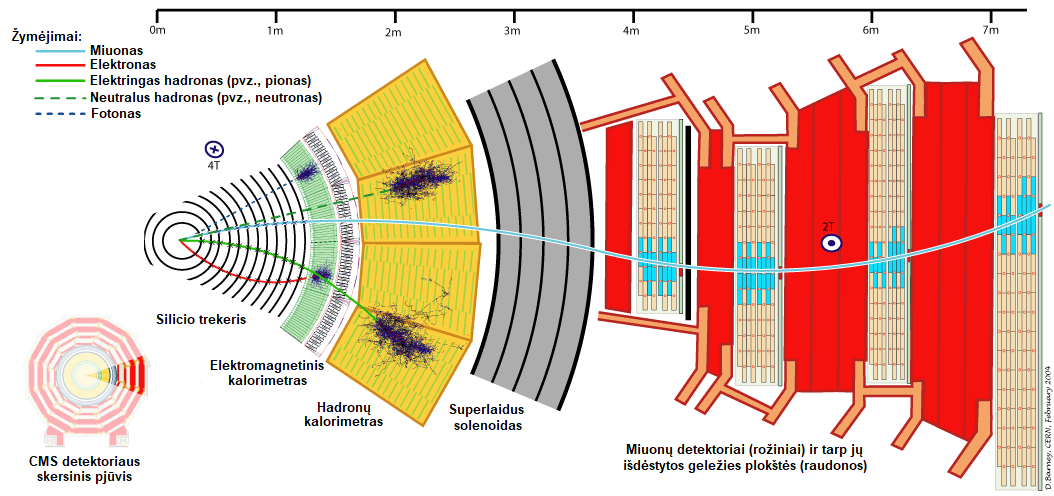
\includegraphics[width=0.85\textwidth]{CMSslice_LT.png}
\tiny (http://ippog.org/resources/2011/cms-slice-july-2010-version)
\end{figure}
\end{frame}

\begin{frame}
\subsection{Partonų pasiskirstymo funkcijos}
\frametitle{Papildoma informacija\\ \small Partonų pasiskirstymo funkcijos}
\begin{itemize}
\item Nuo partonų pasiskirstymo funkcijų tikslumo priklauso visų protonų susidūrimo metu vykstančių procesų teorinių įverčių tikslumas;
\item Partonų pasiskirstymo funkcijos yra tikslinamos pasinaudojant tokių procesų, kaip Drell-Yan procesas eksperimentinio tyrimo rezultatais;
\end{itemize}
\vspace{-0.6cm}
\begin{columns}
\column{0.5\textwidth}
\begin{figure}[H]
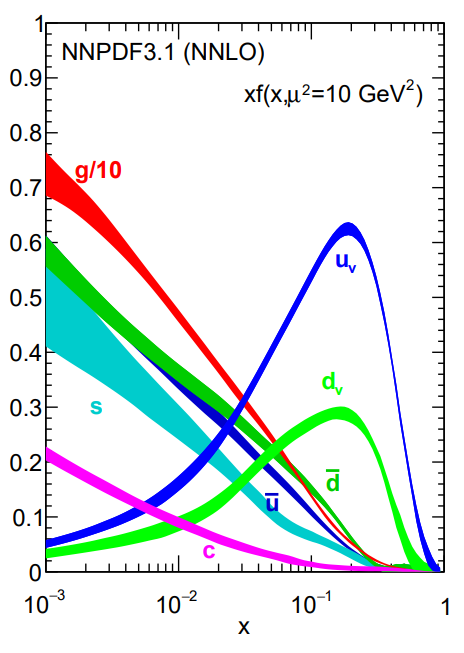
\includegraphics[width=0.62\textwidth]{NNPDF10.PNG}
\end{figure}
\column{0.5\textwidth}
\begin{figure}[H]
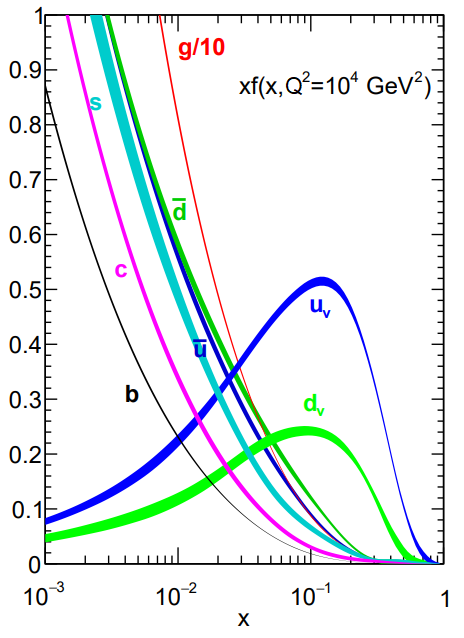
\includegraphics[width=0.62\textwidth]{NNPDF10000.PNG}
\end{figure}
\end{columns}
\tiny (The NNPDF Collaboration. Eur.\ Phys.\ J.\ C77 no.\ 10, 663, 2017.)
\end{frame}

\begin{frame}
\subsection{Invariantinė masė}
\frametitle{Papildoma informacija\\ \small Invariantinė masė}
\begin{itemize}
\item Invariantinė masė -- tai objekto (rimties) masė, kuri nepriklauso nuo atskaitos sistemos;
\item Prilyginus $\mathit{c}=1$, invariantinė masė bet kokioje atskaitos sistemoje apskaičiuojama taip:
\begin{equation*}
\mathit{m}_{\, 0}^{\, 2}=\mathit{E}^{\, 2}-|\vec{\mathit{p}}|^{2} \; ;
\end{equation*}
\item Dviejų dalelių invariantinė masė apskaičiuojama taip:
\begin{equation*}
\mathit{m}_{\, 12}^{\, 2}=(\mathit{E}_{\, 1}+\mathit{E}_{\, 2})^{2}-|\vec{\mathit{p}_{\, 1}}+\vec{\mathit{p}_{\, 2}}|^{2} \; ;
\end{equation*}
\end{itemize}


\end{frame}

\begin{frame}
\subsection{Reakcijų skerspjūviai}
\frametitle{Papildoma informacija}
Protonų susidūrimų energija $\sqrt{\mathit{s}}=13$ $TeV$. Procesų reakcijų skerspjūviai:
\begin{table}[H]
\begin{tabular}{|c|c|}
\hline
Procesas & Reakcijos skerspjūvis (\pb) \\
\hline\hline
$\DYee$ & $8211.73$ \\
\hline
$\mathrm{DY}\!\rightarrow\! \mu\mu$ & $8211.73$ \\
\hline
$\DYtau$ & $8211.73$ \\
\hline
$\ttbar$ & $831.76$ \\
\hline
$\dtW$ & $76.18$ \\
\hline
$\WJets$ & $61526$ \\
\hline
$\WW$ & $118.7$ \\
\hline
$\WZ$ & $47.13$ \\
\hline
$\ZZ$ & $16.523$ \\
\hline
$\gJets$ & $3.65896\cdot10^{5}$ \\
\hline
$\QCD$ & $5.19096\cdot10^{6}$ \\
\hline
\end{tabular}
\end{table}
Integruotas šviesis $\mathit{ee}$ kanalui: $\Lumi=2.26$ \invfb, $\mathit{e\mu}$ kanalui: $\Lumi=2.32$ \invfb.\\
\end{frame}

\begin{frame}
\subsection{Modeliuotų įvykių normavimas}
\frametitle{Papildoma informacija\\ \small Modeliuotų įvykių normavimas}
\begin{itemize}
\item Jeigu įvykių generatoriaus kiekvienam įvykiui priskirti pradiniai svoriai yra vienodi tada modeliuoto įvykio svorį galima apskaičiuoti pagal formulę:
\begin{equation*}
\omega=\frac{\sigma \Lumi}{\mathit{N}} \; ;
\end{equation*}
\item Bendru atveju (ir šiuo atveju):
\begin{equation*}
\omega_{\mathit{i}}^{\mathrm{Piln.}}=\omega_{\mathit{i}}\frac{\sigma \Lumi}{\sum_{\mathit{j}=1}^{\mathit{N}}\omega_{\mathit{j}}} \; ;
\end{equation*}
\end{itemize}
\end{frame}

\begin{frame}
\subsection{Matavimu grįsti triukšmo įvykių įvertinimo metodai}
\frametitle{Papildoma informacija\\ \small Matavimu grįsti triukšmo įvykių įvertinimo metodai}
\textbf{Kontrolinėje srityje}, kurioje dominuoja triukšmo įvykiai apskaičiuotas įvykių skaičius transformuojamas į triukšmo įvykių skaičių \textbf{signalo srityje}.\\
\vspace{0.3cm}
Pagrindiniai matavimu grįsti triukšmo įvykių skaičiaus įvertinimo metodai:
\begin{itemize}
\item Klaidingo atpažinimo metodas\\
Skirtas įvertinti procesams, kuriuose gali susidaryti čiurkšlės (angl. \textit{jets});
\item ABCD metodas\\
Skirtas įvertinti procesams, kuriuose gali susidaryti čiurkšlės;
\begin{block}{$\emu$ metodas}
Skirtas įvertinti procesams, kuriuose susidaro dvi nestabilios dalelės, skylančios į leptonus nepriklausomai;
\end{block}
\item Ir kt.
\end{itemize}
\end{frame}

\begin{frame}
\subsection{Modeliuoto Drell-Yan signalo tikrinimas}
\frametitle{Papildoma informacija\\ \normalsize Modeliuoto Drell-Yan signalo tikrinimas}
\begin{itemize}
\item Modeliuotas Drell-Yan signalo spektras buvo išskirstytas po kelis skirtingus failus;
\item Kad skirtingų failų sandūrose perėjimas būtų tolygus, įvykius reikėjo teisingai sunormuoti;
\end{itemize}
\end{frame}

\begin{frame}
\subsection{ee įvykių atranka}
\frametitle{Papildoma informacija\\ \small $\ee$ įvykių atranka}
Elektronų poros įvykių atrankos reikalavimai:
\begin{enumerate}
\item Trigeris \texttt{Ele23\_WPLoose} (elektronas, su skersiniu impulsu, didesniu, negu $23$ $\mathrm{GeV}$);
\item Du elektronai, atitinkantys \textit{MediumID} reikalavimus;
\item Detektoriaus dalies, į kurią pataikė elektronas, pseudosparta $|\eta_{\mathrm{SC}}|<2.5$, išskyrus $1.4442<|\eta_{\mathrm{SC}}|<1.566$;
\item Greitesniojo elektrono skersinis impulsas $\pT^{\mathrm{Gr.}}>30$ $\mathrm{GeV}$, lėtesniojo $\pT^{\mathrm{Lėt.}}>10$ $\mathrm{GeV}$;
\end{enumerate}
\end{frame}

\begin{frame}
\subsection{emu įvykių atranka}
\frametitle{Papildoma informacija\\ \small $\emu$ įvykių atranka}
Elektrono ir miuono įvykių atrankos reikalavimai:
\begin{enumerate}
\item Trigeris \texttt{Mu8\_Ele17} (miuonas, su skersiniu impulsu, didesniu, negu $8$ $\mathrm{GeV}$ ir elektronas, su skersiniu impulsu, didesniu, negu $17$ $\mathrm{GeV}$);
\item Vienas elektronas, atitinkantis \textit{MediumID} kriterijų;
\item Vienas miuonas, atitinkantis \textit{TightID} kriterijų;
\item Elektrono skersinis impulsas $\pT^{\mathit{e}}>25$ $\mathrm{GeV}$, miuono $\pT^{\mu}>15$ $\mathrm{GeV}$;
\item Detektoriaus dalies, į kurią pataikė elektronas pseudosparta $|\eta_{\mathrm{SC}}|<2.5$, išskyrus $1.4442<|\eta_{\mathrm{SC}}|<1.566$;
\item Miuono pseudosparta $|\eta_{\mu}|<2.4$;
\item Miuono atskirumas trekeryje $\mathit{I}_{\mathrm{Trk.}}<0.1$ arba \textit{dalelių srauto} algoritmo apskaičiuotas miuono atskirumas $\mathit{I}_{\mathrm{PF}}<0.1$;
\end{enumerate}
\end{frame}

\begin{frame}
\subsection{Normavimas pagal protonų susidūrimų tankį I}
\frametitle{Papildoma informacija\\ \normalsize Normavimas pagal protonų susidūrimų tankį}
Protonų susidūrimo tankio pasiskirstymas modeliavime ir matavime nesutapo. Todėl modeliuotiems įvykiams buvo priskirti papildomi svoriniai daugikliai. Jie buvo skaičiuojami kaip pasiskirstymų santykis, aproksimuotas dvipusio Gauso pasiskirstymo funkcija.

\begin{equation*}
\mathit{F}^{\mathrm{\;sant.}}(\mathit{N}_{\mathrm{PV}})=\frac{\mathit{F}^{\,\mathrm{Data}}(\mathit{N}_{\mathrm{PV}})}{\mathit{F}^{\,\mathrm{MC}}(\mathit{N}_{\mathrm{PV}})}\cdot \frac{\int \mathit{F}^{\,\mathrm{MC}}(\mathit{N}_{\mathrm{PV}}) \mathrm{d}\mathit{N}_{\mathrm{PV}}}{\int \mathit{F}^{\,\mathrm{Data}}(\mathit{N}_{\mathrm{PV}}) \mathrm{d}\mathit{N}_{\mathrm{PV}}}
\end{equation*}

\begin{equation*}
\overline{\mathit{F}}^{\mathrm{\;sant.}}(\mathit{N}_{\mathrm{PV}})=
\begin{cases} \mathit{A}\cdot \exp\left(-\frac{(\mathit{x}-\mathit{x}_{\,0})^{2}}{2\sigma_{1}^{2}}\right), & \mbox{kai } \mathit{x}<\mathit{x}_{\,0} \vspace{0.2cm} \\ 
\mathit{A}\cdot \exp\left(-\frac{(\mathit{x}-\mathit{x}_{\,0})^{2}}{2\sigma_{2}^{2}}\right), & \mbox{kai } \mathit{x}\geqslant \mathit{x}_{\,0} \end{cases}
\end{equation*}
\end{frame}

\begin{frame}
\subsection{Normavimas pagal protonų susidūrimų tankį II}
\frametitle{Papildoma informacija\\ \normalsize Normavimas pagal protonų susidūrimų tankį}
\end{frame}

\begin{frame}
\subsection{Normavimas pagal protonų susidūrimų tankį III}
\frametitle{Papildoma informacija\\ \normalsize Normavimas pagal protonų susidūrimų tankį}
Pirminių viršūnių skaičiaus pasiskirstymas po pernormavimo:
\end{frame}

\begin{frame}
\subsection{Dalelių srauto atskirumas}
\frametitle{Papildoma informacija\\ \normalsize \textit{Dalelių srauto} atskirumas}
Buvo pastebėta, kad pritaikius papildomus reikalavimus miuono atskirumui, apskaičiuojamam naudojantis \textit{dalelių srauto} algoritmu, galima sumažinti $\WJets$ įvykių, praeinančių $\emu$ atranką, skaičių:
\tiny
\begin{equation*}
\mathit{I}^{\mathrm{rel.}}_{\mathrm{PF}}= \frac{1}{\pT} 
\left[ \sum_{\Delta \mathit{R}<0.3} \pT^{\mathrm{Ch.\;hadron}}+\mathrm{max}
\left( \sum_{\Delta \mathit{R}<0.3} \pT^{\mathrm{N.\;hadron}}+\sum_{\Delta \mathit{R}<0.3} \pT^{\gamma}-\Delta \beta \sum_{\Delta \mathit{R}<0.3} \pT^{\mathrm{PU}} \, ,\;\; 0 \right) \right] \; \mathrm{;}
\end{equation*}

\end{frame}

\begin{frame}
\subsection{Modeliuotų įvykių atrankos rezultatai I}
\frametitle{Papildoma informacija\\ \small Įvykių atrankos rezultatai}
Gautas $\ee$ invariantinės masės spektras:\\
\centering
\vspace{0.3cm}
\end{frame}

\begin{frame}
\subsection{Modeliuotų įvykių atrankos rezultatai II}
\frametitle{Papildoma informacija\\ \small Įvykių atrankos rezultatai}
Gautas $\emu$ invariantinės masės spektras:\\
\centering
\vspace{0.3cm}
\end{frame}

\begin{frame}
\subsection{Triukšmų įskaitymas}
\frametitle{Papildoma informacija\\ \small Panašių į $\emu$ įvykių (\ltq{$\emu$ triukšmų}) įskaitymas taikant $\emu$ metodą}
\begin{equation*}
\mathit{N_{ee}^{\mathrm{Įvert.}}}=\frac{\mathit{N_{ee}^{\mathrm{MC}}}}{\mathit{N_{e\mu}^{\mathrm{MC}}}}\mathit{N_{e\mu}^{\mathrm{Data}}} \; ;
\end{equation*}
\begin{itemize}
\item Problema: tarp atrinktų $\emu$ įvykių yra ir $\emu$ triukšmo įvykių: $\WJets$, $\gJets$, $\QCD$, $\WZ$, $\ZZ$;
\item Jie yra netinkami $\emu$ metodui;
\item Į šių triukšmų egzistavimą buvo bandoma atsižvelgti įvedant daugiklį $1/(1+\mathit{R})$, kur
\begin{equation*}
\mathit{R}=\frac{
\mathit{N}_{\WJets}^{\, \emu , \; \mathrm{MC}}+
\mathit{N}_{\gJets}^{\, \emu , \; \mathrm{MC}}+
\mathit{N}_{\WZ}^{\, \emu , \; \mathrm{MC}}+
\mathit{N}_{\ZZ}^{\, \emu , \; \mathrm{MC}}
}{
\mathit{N}_{\WW}^{\, \emu , \; \mathrm{MC}}+
\mathit{N}_{\tW}^{\, \emu , \; \mathrm{MC}}+
\mathit{N}_{\tbarW}^{\, \emu , \; \mathrm{MC}}+
\mathit{N}_{\ttbar}^{\, \emu , \; \mathrm{MC}}+
\mathit{N}_{\DYtau}^{\, \emu , \; \mathrm{MC}}
} \;\; ;
\end{equation*}
\item Buvo išbandytas ir variantas, kai įskaitoma tik $\WJets$ (dominuojančio triukšmo) įtaka;
\end{itemize}
\end{frame}

\begin{frame}
\subsection{Paklaidų įvertinimas}
\frametitle{Papildoma informacija\\ \small Paklaidų įvertinimas}
\begin{itemize}
\item CERN LHC vykstantys protonų susidūrimo įvykiai yra Puasono įvykiai;
\item CMS detektoriaus užregistruotų įvykių statistinė paklaida skaičiuojama kaip kvadratinė šaknis iš įvykių skaičiaus;
\item Modeliuotų įvykių statistinė paklaida skaičiuojama kaip kvadratinė šaknis iš modeliuotų įvykių svorių kvadratų sumos:
\begin{equation*}
\Delta \mathit{N}_\mathrm{MC} = \sqrt{\sum_{\mathit{i}=1}^{\mathit{n}}\mathit{w_{i}}^{2}} \;\; ;
\end{equation*}
\item Įvykių skaičiaus sisteminė paklaida skaičiuojama kaip skirtumo tarp pasiskirstymų, gautų naudojant skirtingus parametrus, modulis:
\begin{equation*}
\Delta \mathit{N}(\mathit{m}_{\ee}) = \left| \, \mathit{N}(\mathit{m}_{\ee} | \mathrm{p}_{1}) - \mathit{N}(\mathit{m}_{\ee} | \mathrm{p}_{2}) \, \right| \; ;
\end{equation*}
\end{itemize}
\end{frame}

\begin{frame}
\subsection{Pasiskirstymų sutapimas}
\frametitle{Papildoma informacija\\ \small Pasiskirstymų sutapimas}
Nesutapimą tarp įverčio ir modeliavimo aprašantis dydis $\chi^{2}/\mathit{n}_{\mathrm{\, l. \, l.}}$ su $\mathit{Z}$ bozono rezonansu siejamoje srityje:
\begin{itemize}
\item Modeliuotam įverčiui: $67.42$;
\item $\emu +$modeliuotam įverčiui: $66.54$;
\item Sumažėjimas $1.3\%$;
\end{itemize}
\medskip
$\chi^{2}$ skaičiuojamas taip:
\begin{equation}
\chi^{2} = \sum_{\mathit{i}=1}^{\mathit{n}} \frac{ \left( \mathit{N}_{\mathit{i}}^{\,\mathrm{Data}} - \mathit{N}_{\mathit{i}}^{\,\mathrm{Įvert.}} \right) ^{2} }
{ \left( \Delta \mathit{N}_{\mathit{i}}^{\,\mathrm{Data}} \right) ^{2} }
\end{equation}
\end{frame}

\begin{frame}
\subsection{Antrinės išvados}
\frametitle{Papildomos išvados}
\begin{itemize}
\item Didelių energijų fizikos duomenų analizės darbas reikalauja daug laiko ir kruopštumo.
\item Labai didelio tikėtinumo triukšmo įvykiai (pvz., vienam $\DYee$ įvykiui tenka $632$ $\QCD$ įvykiai) su maža tikimybe praeina atrankos kriterijus, todėl jų pasiskirstymą sunku pakankamai tiksliai modeliuoti. Tai nulemia \ltq{pikų} atsiradimą histogramose.
\item Pakeitus miuonų atrankos reikalavimus galima sumažinti $\emu$ atranką praeinančių $\WJets$ įvykių skaičių.
\item Parašyti protonų susidūrimo įvykių atrankos, $\emu$ metodo skaičiavimų bei grafikų brėžimo programiniai kodai su minimaliomis korekcijomis galės būti taikomi ir atliekant naujesnių metų CMS duomenų analizę.
\end{itemize}
\end{frame}

\end{document}
